\documentclass[12pt]{article}
%\usepackage{tkiz}

\usepackage[utf8]{inputenc}
\usepackage[french]{babel}
\usepackage{amsmath,amsthm,amsfonts,amssymb}
\usepackage{lmodern}
\usepackage[top=2.4cm,bottom=2.4cm,left=2cm,right=2cm]{geometry}
\usepackage{hyperref}
\usepackage{multicol}
\usepackage{enumitem}
\usepackage{listings}
\usepackage[dvipsnames]{xcolor}
\usepackage{tikz}
\author{MABROUK Fayez}
\date{N°etudiant : 22213839}
\title{{\bf  Génie logiciel} \\
	Rendu de TD06\\
	{\small L3 Informatique appliquée 2022-2023} \\
	{\it \small }}

\begin{document}
	\maketitle
	\newpage
	\section{Cas d'utilisation simple}
	Vous devez, à l’aide de la solution logicielle de votre choix , proposer un diagramme de cas d’utilisation et répondre aux questions dans les
	scénarios qui suivent. Dans chaque diagramme, le nom du système devra être suivi par votre nom de
	famille en majuscules (e.g. Livraison à domicile LOBRY) :
	\begin{itemize}
		\item[1. ] On souhaite développer un outil de gestion numérique d’une bibliothèque municipale. On
		souhaite modéliser les cas d’utilisation suivants :
		\begin{itemize}
			\item[a. ] À la réception d’un ou plusieurs nouveaux livres, l’enregistrement de ceux-ci dans la
			base de données.
			\begin{itemize}
				\item[i. ] Quels sont les acteurs, éventuellement primaires/secondaires ?\\
				Bibliothécaire.
				\item[ii. ] Quel est le système ?\\
				Gestion de bibliothèque.
				\item[iii. ] Dessinez le cas d’utilisation: 
				%1..* pas 1..N
				\right) 
			\end{itemize}
		\item[b. ] L’emprunt d’un ou plusieurs livres. On notera que le nombre maximum de livres
		pouvant être empruntés est de 5.
		\begin{itemize}
			\item[i. ] Quels sont les acteurs, éventuellement primaires/secondaires ?\\
			Primaire : emprunteur.\\
			Secondaire : Bibliothécaire.
			\item[ii. ] Quel est le système ?\\
			Gestion de bibliothèque.
			\item[iii. ] Dessinez le cas d’utilisation:
			\begin{figure}[!hbtp]
				%\centering
				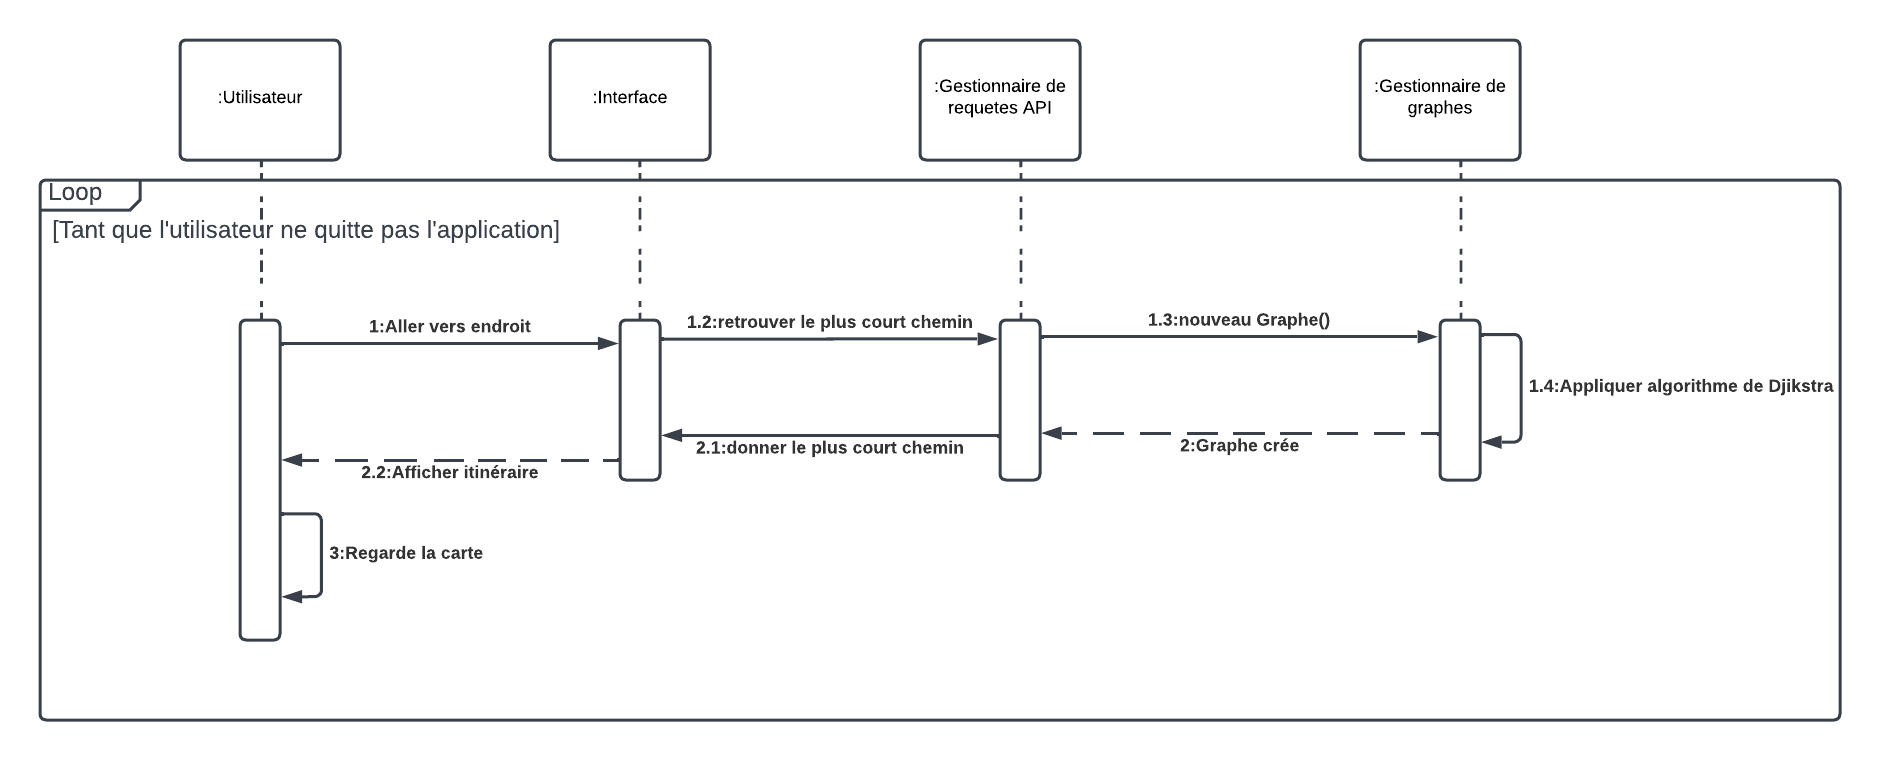
\includegraphics[scale=0.75]{capture2.PNG}
				%\caption{Légende de l'image}
			\end{figure}
			
		\end{itemize}
		\end{itemize}
	\item[2. ] On souhaite modéliser le fonctionnement d’un restaurant dans les cas suivants :
	\begin{itemize}
		\item[a. ] À la prise de commande du client.
		\begin{itemize}
			\item[i. ] Quels sont les acteurs, éventuellement primaires/secondaires ?\\
			Primaire : Client.\\
			Secondaire : Serveur, cuisinier.
			\item[ii. ] Quel est le système ?\\
			Restaurant.
			\item[iii. ] Dessinez le cas d’utilisation:
				\begin{figure}[!hbtp]
				%\centering
				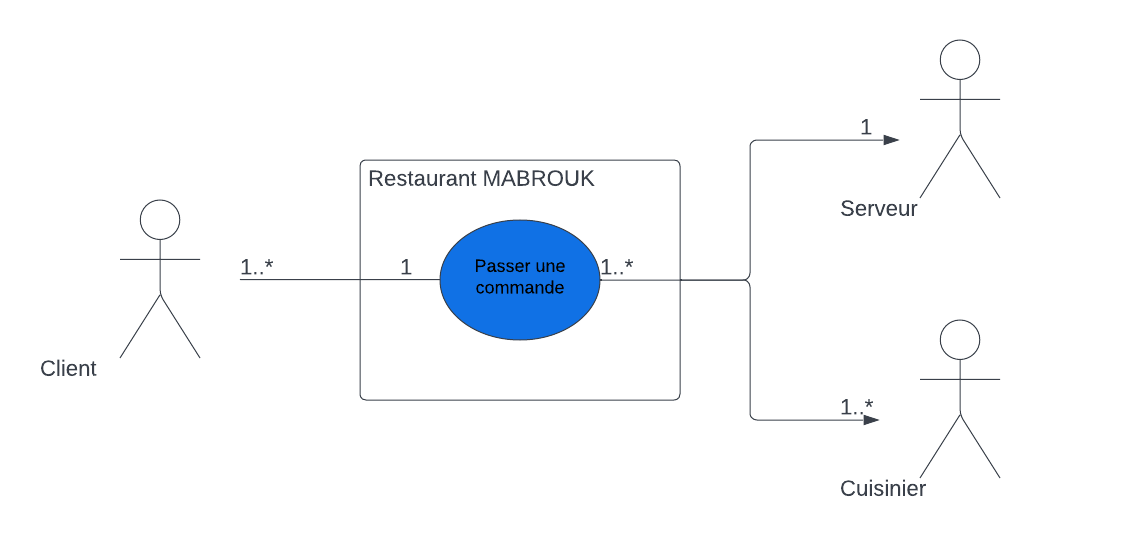
\includegraphics[scale=0.75]{capture3.PNG}
				%\caption{Légende de l'image}
			\end{figure}
		\end{itemize}
	\item[b. ] Au paiement du client.
	\begin{itemize}
		\item[i. ] Quels sont les acteurs, éventuellement primaires/secondaires ?\\
		Primaire : Client.\\
		Secondaire : Serveur, société de paiement.
		\item[ii. ] Quel est le système ?\\
		Restaurant.
		\item[iii. ] Dessinez le cas d’utilisation:
			\begin{figure}[!hbtp]
			%\centering
			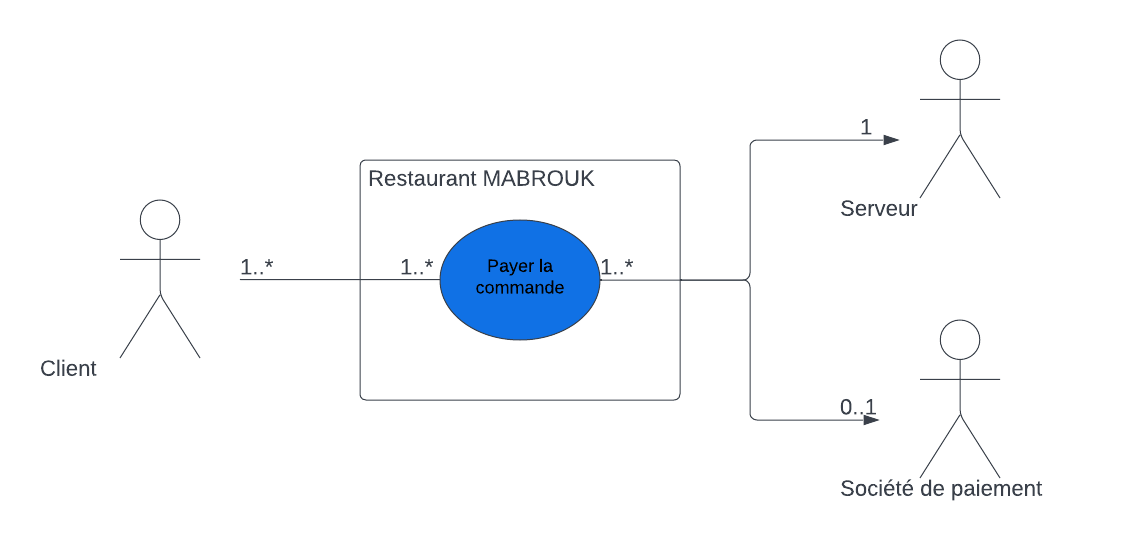
\includegraphics[scale=0.75]{capture4.PNG}
			%\caption{Légende de l'image}
		\end{figure}
	\end{itemize}
	\end{itemize}
	\end{itemize}
\section{Projet fil rouge}
\begin{itemize}
	\item[1. ] Individuellement, listez les risques (attention à la définition d’un risque) liés à votre projet fil
	rouge (écrivez-les sur votre compte-rendu).\\
	\begin{itemize}
		\item Mauvais marketing : Difficultés à bien commercialiser l’application.
		\item Mauvaise embauche : un développeur n’a pas les connaissances requises pour effectuer une tâche dans le temps donné.
		\item Faille de sécurité : Une implémentation hâtive de la partie backend de l’application peut entraîner des failles de sécurité ce qui mettrait en danger les données privées des utilisateurs.
		\item Panne de la base de données : une mauvaise conception de la BDD peut conduire à un défaut ultérieur qui peut causer la perde des données des utilisateurs.
		\item Evolution des technologies : API obsolètes.
		\item  Problème externes (guerre dans le monde, pandémie mondiale, coupure de courant, etc...).
	\end{itemize}
\item [2. ] Individuellement, classifiez ces risques selon les 3 classifications vues en cours (écrivez-les sur
votre compte-rendu).\\
\\
\begin{tabular}{|p{3.5cm}|p{5cm}|} 
	\hline  
	\centering Types de risques & \raggedright  Classification1 \tabularnewline  
	\hline
	\raggedleft humains&  Mauvais marketing : Difficultés à bien commercialiser l’application. \tabularnewline  
	\hline  
	\raggedleft Gestions & Mauvaise embauche : un développeur n’a pas les connaissances requises  pour effectuer une tâche dans le temps donné. \tabularnewline  
	\hline  
	\raggedleft Techniques & Evolution des technologies : API obsolètes. \tabularnewline 
	\hline 
\end{tabular}\\
\begin{tabular}{|p{3.5cm}|p{5cm}|} 
	\hline  
	\centering Types de risques & \raggedright  Classification2 \tabularnewline  
	\hline
	\raggedleft Procédés&  \tabularnewline  
	\hline  
	\raggedleft Qualités & Faille de sécurité : Une implémentation hâtive de la partie backend de l’application peut entraîner des failles de sécurité ce qui mettrait en danger les données privées des utilisateurs. \tabularnewline  
	\hline  
	\raggedleft Viabilités & Panne de la base de données : une mauvaise conception de la BDD peut conduire à un défaut ultérieur qui peut causer la perde des données des utilisateurs.. \tabularnewline 
	\hline 
\end{tabular}\\
\begin{tabular}{|p{3.5cm}|p{5cm}|} 
	\hline  
	\centering Types de risques & \raggedright  Classification3 \tabularnewline  
	\hline
	\raggedleft Impact sur tout le projet& Problème externes (guerre dans le monde, pandémie mondiale, coupure de courant, etc...)
	  \tabularnewline  
	\hline  
\end{tabular}
	\item[3. ] En groupe, confrontez vos listes et classifications et proposez un document unique au
	groupe, à mettre à la suite de votre liste individuelle.\\
	\\
	\textbf{Groupe :} MABROUK Fayez , PHAN Dao , AHMED-ZAID Macyl\\
	\\
	\begin{tabular}{|p{3.5cm}|p{8cm}|} 
		\hline  
		\centering Types de risques & \raggedright  Classification1 \tabularnewline  
		\hline
		\raggedleft humains&  - Problème humain, arrêt maladie ou encore acte de décès d’un proche
		
		-Problèmes entre employés (développeurs) ce qui peut conduire à une mauvaise entente entre eux et cela risque la contre-performance d’un des employés
		
		- Compétence techniques insuffisantes d’un employé
		
		- Risque d’abandon (de démission)
		 \tabularnewline  
		\hline  
		\raggedleft Gestions & - Allocation du budget insuffisante
		
		- Mauvaise embauche des employés en fonctions des compétences techniques requises
		
		-Une analyse des besoins et d’exigences mal réfléchie 
		
		- Mauvais marketing
		
		-Mauvaise répartition de tâches entre développeurs
		
		- Personnel en sous-effectifs, mauvaise prise en compte des besoins de conceptions et de maintenances
		 \tabularnewline  
		\hline  
		\raggedleft Techniques & - Problème de performance finale du logiciel
		
		- Evolution des technologies (API obsolètes)
		
		- Une mauvaise utilisation d’un gestionnaire de    version (Git, Svn)
		. \tabularnewline 
		\hline 
	\end{tabular}\\
	\begin{tabular}{|p{3.5cm}|p{8cm}|} 
		\hline  
		\centering Types de risques & \raggedright  Classification2 \tabularnewline  
		\hline
		\raggedleft Procédés&  - Choix d’un cycle de vie incompatible avec la gestion du projet\tabularnewline  
		\hline  
		\raggedleft Qualités & - Failles de sécurité
		
		- Protection des données des utilisateurs
		
		- Problèmes d’affichage des interfaces sur différents appareils
		
		- Non-respect des normes RGPD
		
		- Bug logiciels
		
		- Fonctionnalités implémentées contre-intuitives
		 \tabularnewline  
		\hline  
		\raggedleft Viabilités & Problèmes pour la maintenance
		
		- Mauvaise performance logiciel
		
		- Panne des BDD (perte de donnés)
		
		- Surchage des serveurs
		\tabularnewline 
		\hline 
	\end{tabular}\\
	\begin{tabular}{|p{3.5cm}|p{8cm}|} 
		\hline  
		\centering Types de risques & \raggedright  Classification3 \tabularnewline  
		\hline
		\raggedleft Impact sur tout le projet& - Problème externes (guerre dans le monde, pandémie mondiale, coupure de courant, etc...)
		\tabularnewline  
		\hline  
	\end{tabular}
	
	
\end{itemize}

\end{document}